\documentclass[oneside,12pt]{book}
% oneside - onesided print

%\usepackage[czech]{babel}
\usepackage[utf8]{inputenc}
\usepackage[a4paper,width=150mm,top=25mm,bottom=30mm]{geometry}
\usepackage[backend=biber,style=numeric,sorting=none]{biblatex}
\usepackage{setspace, enumitem, amsmath, amsfonts, amsthm, amssymb, graphicx, soul, float, multirow, hyperref}
\usepackage{xcolor, listings, csquotes, wrapfig, tabularx, forest, subcaption}
\usepackage[bottom]{footmisc}

% Page number at the end of page and no chapter name in the header
\pagestyle{plain}

\setstretch{1.5}

\setcounter{secnumdepth}{3}
\setcounter{tocdepth}{4}

\bibliography{references}

\definecolor{keywords}{rgb}{0,0,0.7}

\lstset{
columns=fullflexible,
keywordstyle=\color{keywords},
frame=lines,
language=Python,
%numbers=left,
%numbersep=5pt,
basicstyle=\small,
%numberstyle=\footnotesize\color{Gray},
commentstyle=\it\footnotesize\color{Gray}
}

\newenvironment{boldenv}{\bfseries}{}

\newcommand\norm[1]{\left\lVert#1\right\rVert}

% Centered X column in tabularx environment
\newcolumntype{Y}{>{\centering\arraybackslash}X}

\begin{document}
    \pagenumbering{gobble}

    \begin{titlepage}
    \begin{boldenv}
        \begin{center}
            \vspace*{20pt}
            \LARGE
            University of West Bohemia \\
            \vspace*{5pt} Faculty of Applied Sciences  \\
            \vspace*{5pt} Department of Cybernetics\\

            \vfill
            \huge
            MASTER THESIS

            \vfill

        \end{center}
        \begin{flushleft}
            \Large
            PILSEN, 2020
            \hfill
            JAN BENEŠ
        \end{flushleft}
    \end{boldenv}
\end{titlepage}

    Před svázáním místo této stránky \fbox{vložit zadání práce} s podpisem děkana.
    \newpage

    \vspace*{20pt}
\begin{center}
    \underline{Declaration of Authorship}
\end{center}

I, Jan Beneš, declare that this thesis titled, “Automatic face recognition using neural networks” and the work 
presented in it are my own.

I confirm that:
\begin{itemize}
    \item Where I have consulted the published work of others, this is always clearly attributed.
    \item Where I have quoted from the work of others, the source is always given.
    With the exception of such quotations, this thesis is entirely my own work.
    \item I have acknowledged all main sources of help.
\end{itemize}

    \newpage

    \vspace*{20pt}
\noindent
{\LARGE
\textbf{Acknowledgements}
}
\vspace*{0.5em}

I would like to express my gratitude and appreciation to Ing. Ivan Gruber for his guidance throughout the project.

Likewise, I would like to thank my supervisor Ing. Marek Hrúz, Ph.D. for providing me with invaluable feedback.

My gratitude also goes to MetaCentrum VO for allowing  me to use their computational resources.

Finally, I have to thank my family for supporting me in the pursuit of my studies.

    \newpage

    \section*{Abstract}
The goal of this study is to design and implement an end-to-end facial recognition system.
The first part is focused on a general overview of modern methods followed by an in-depth description of
state-of-the-art research of loss functions.
The emphasis is being put on the ArcFace loss as it is the research which forms the basis of the facial recognition
system implemented in this thesis.
The second part deals with the design and implementation of the system.
The end of the text contains a comparison with a commercial algorithm.
The performance was evaluated on a dataset which was created from the recordings of evening news on the czech public
television broadcast (Česká Televize).

\vspace{1cm}

\subsection*{Key words}
Machine learning, facial recognition, identification, verification, convolutional neural networks, loss functions,
ArcFace

\vfill

\section*{Abstrakt}
Cílem této práce je návrh a implementace systému rozpoznávání obličeje.
V první části je poskytnut přehled moderních metod, na který navazuje podrobný rozbor výzkumu ztrátových funkcí.
Důraz je kladen na ztrátovou funkci ArcFace.
Tato funkce byla použita při trénování modelu, jenž tvoří jádro systému implementovaného v rámci této práce.
Druhá část práce obsahuje návrh a popis implementace systému.
V závěru je systém porovnán s komerčním algoritmem.
Vyhodnocení proběhlo na datasetu, jenž byl vytvořen ze záznamu večerních zpráv České Televize.

\vspace{1cm}

\subsection*{Klíčová slova}
Strojové učení, rozpoznávání obličeje, identifikace, verifikace, konvoluční neuronové sítě, ztrátové funkce, ArcFace

    \tableofcontents

    \chapter{Introduction}\label{ch:introduction}

\section{Objectives}\label{sec:objectives}
The objectives of this text are:
\begin{enumerate}
    \item to provide an overview of modern facial recognition methods;
    \item to implement the state-of-the-art algorithm;
    \item to evaluate the system's performance on appropriate benchmark dataset;
    \item to compare the results with commercial algorithm.
\end{enumerate}

\section{Outline}\label{sec:outline}

    \pagenumbering{arabic}

    \chapter{Convolutional Neural Networks}\label{ch:cnn}
Convolutional Neural Networks (CNNs) are a group of models which allow for efficient training on high dimensional data.
This is especially useful in the field of computer vision as image data is fundamentally high dimensional.

\begin{figure}[H]
    \centering
    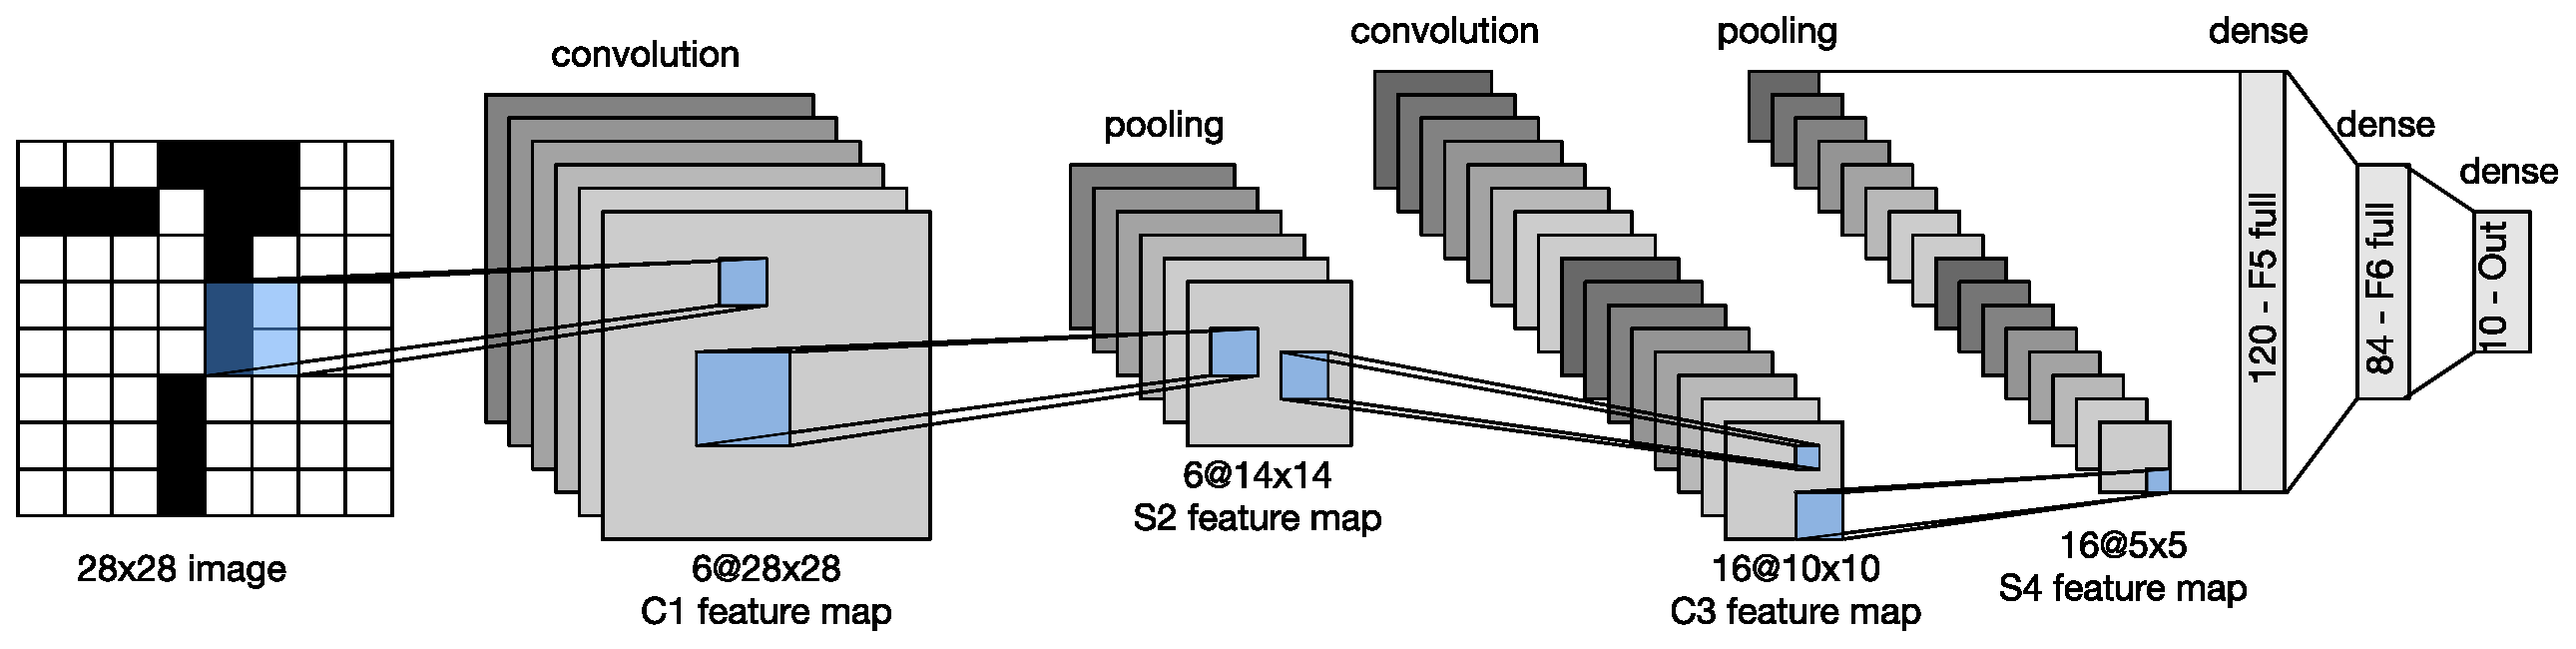
\includegraphics[width=\columnwidth]{images/cnn/lenet.eps}
    \caption{Example of CNN model (LeNet 5)~\cite{CNN}}
    \label{fig:cnn}
\end{figure}

The image~\ref{fig:cnn} is an illustration of one of the oldest CNN models \textit{LenNet 5} which was used for
handwritten character recognition.
As we can see, there are many layers stacked in the model's architecture.
This is typical for CNNs and it's a reason why CNNs belong to the class of machine learning methods called
\textit{deep learning}\footnote{Set of machine learning models with
\textit{credit assignment path (CAP)} higher than 2.
The CAP is the chain of transformations from input to output.}
Usually there are three layer types in the CNN model: \textit{dense}~\ref{sec:dense},
\textit{convolutional}~\ref{sec:convolutional} and \textit{pooling}~\ref{sec:pooling}.

\section{Dense layer}\label{sec:dense}
Dense layer is the simplest type of layer present in CNN models.
Its output is determined simply by multiplication of \textit{inputs} (x) with \textit{weight matrix}
(denoted V in~\ref{eq:dense}, also called kernel) and addition of \textit{bias} (u).

\begin{equation}
    \label{eq:dense}
    h[i, j] = u[i,j] + \sum_{a,b} V[i,j,a,b] \cdot x[i+a,j+b]
\end{equation}

Now let's imagine, that we have greyscale image which is 256 pixel wide and high as an input.
If we flatten the image to a vector, we get input with $256\cdot256 = 65536$ dimensions.
Even if we do aggressive reduction to 1000 hidden dimensions, we end up with ~65 million parameters.
This makes dense layer impractical when dealing with imagery and that's when convolution~\ref{sec:convolutional} comes
into play.

\section{Convolutional layer}\label{sec:convolutional}
As I hinted in the previous section, the main objective of convolutional layer is to decrease the amount of parameters
needed.
This feat was achieved by application of two principles: \textit{invariance}~\ref{subsec:invariance} and
\textit{locality}~\ref{subsec:locality}.

\subsection{Invariance principle}\label{subsec:invariance}
The core of invariance principle is reuse of the weights.
This is achieved by application of the weights on one part of the image, shifting the weights by a predetermined set
of pixels (called stride) and then applying the weights again.
We can have a look at equation~\ref{eq:denseinv} too see how the original equation~\ref{eq:dense} changes.

\begin{equation}
    \label{eq:denseinv}
    h[i, j] = u + \sum_{a,b} V[a,b] \cdot x[i+a,j+b]
\end{equation}

As is to be expected, bias \textit{u} and the weight matrix \textit{V} are no longer dependent upon the image
coordinates \textit{(i, j)}.
As an example we can think of an airplane detection algorithm whose objective is to find whether there is an airplane
in arbitrary location of the scene.
We would do that by sliding one set of weights describing the airplane over the image.
The algorithm would classify the scene with high impulse response as containing the airplane.
This intuitively makes a lot of sense.

This type of invariance is called \textit{translational invariance}.

\subsection{Locality principle}\label{subsec:locality}
Another principle used in CNNs is so called \textit{locality principle}.
This principle suggests, that we do not need to look far away from \textit{(i,j)} to gain valuable information about
what is going on in that particular location.
This is achieved, mathematically speaking, by limiting \textit{a} and \textit{b} to a range $\Delta$.

\begin{equation}
    \label{eq:denseinvloc}
    h[i, j] = u + \sum_{a=-\Delta}^{\Delta} \sum_{b=-\Delta}^{\Delta} V[a,b] \cdot x[i+a,j+b]
\end{equation}

Equation~\ref{eq:denseinvloc} is the final form describing the convolution layer.

\subsection{Padding}\label{subsec:padding}
To avoid loss of information at the edges of the image we usually use a method called \textit{padding}.
This technique increases the image dimension by pixel addition around the original image.
There are few padding variants which are differentiated by the value of the new pixels.
The most common ones are \textit{zero padding} and \textit{reflective padding}.
The first mentioned type, as the name implies, sets the new pixels to zero.
The second one is more sophisticated and consists in mirroring of the neighboring pixels.

\section{Pooling layer}\label{sec:pooling}



    \chapter{Facial Recognition}\label{ch:face-rec}
Facial recognition is a task of verifying or identifying a person from digital image/video.

As I mentioned in the definition, there are two main subtasks~\cite{FaceRec}:
\begin{enumerate}
    \item \textbf{Verification} deals with verifying whether the person in the image is who he claims he is.
    Typical modern use case of verification is smartphone unlocking with face.
    An example of such system is Face ID developed by Apple Inc.

    \item \textbf{Identification} is a task of matching a person to an identity.
    To formulate it in another way, the goal of identification is to give us an answer to the question of who the person
    in the image is.
\end{enumerate}

\section{Pipeline}\label{sec:pipeline}

Facial recognition pipeline\footnote{A chain of processing elements, arranged so that the output of each element is the
input of the next.} usually has the following four steps:
\begin{enumerate}
    \item The first on is \textbf{face detection} and it deals with determination of face location within the image.
    The output of the algorithm is usually face coordinates and facial landmarks.
    Landmarks are a set of coordinates marking important points of the face (eyebrows, nose, mouth, \ldots).
    The knowledge of these points is a necessity for the following step.
    \item \textbf{Face alignment} is a task of changing the face position in such a way that it resembles the position
    of faces on which the feature extraction model was trained.
    In most of the instances this step improves the accuracy.
    \item \textbf{Feature extraction} is a process of computing a feature vector\footnote{A feature vector is a vector
    that contains information describing an object's important characteristics.} of the face.
    Architecture of models used for feature extraction is described in section~\ref{sec:mod-methods}.
    \item \textbf{Feature matching} uses feature vector from the previous task to identify the person in the image.
    The algorithm uses a database of pre-computed feature vectors and compares them to the newly extracted one.
    The identity associated with the feature vector which has the smallest distance from the extracted one is
    considered to be the identity of the person in the image.
\end{enumerate}

\section{Datasets}\label{sec:datasets}
In this section I will briefly describe datasets used for training and evaluation of facial recognition models.
There are too many different datasets used in practice.
For this reason I will focus only on those mentioned in this text.

\subsection{LFW}\label{subsec:lfw}
LFW is an acronym for Labeled Faces in the Wild.
The dataset contains 13,000 images and 1680 identities.
Every identity is represented by at least two samples.
The faces were detected by Viola-Jones face detector\footnote{Real-time object detection framework.}.

There are now four publicly used versions of the dataset.
These versions are differentiated by the type of preprocessing (different methods of alignment) applied to the images.

\subsection{YTF}\label{subsec:ytf}
\subsection{MS-Celeb-1M}\label{subsec:ms1m}

\section{Overview of Modern Methods}\label{sec:mod-methods}
In this section I am about to provide an overview of modern methods/models used for facial recognition.
Models based on CNN architecture~\ref{ch:cnn} achieve state-of-the-art results which is the reason why CNNs dominate the
field of facial recognition and the field of computer vision as a whole now.

Innovations made in the field of computer vision are usually applicable to the subfield of facial recognition as well.
This is manifested in usage of the same model architectures (ResNet~\ref{subsubsec:resnet},
InceptionNet~\ref{subsubsec:inceptionnet}, \ldots) in general image classification as well as in facial recognition.
On the other hand there is a lot of innovation going on in the design of loss functions which work especially well
when used for model training\footnote{Machine learning task of learning a function that maps an input to an output
based on example input-output pairs.} in facial recognition tasks.
This is the reason why this section is divided in two parts: \textit{models}~\ref{subsec:models} and
\textit{loss functions}~\ref{subsec:loss-functions}.

\subsection{Models}\label{subsec:models}
There are two main approaches of training CNNs for face recognition.

The first one is to train a multi-class classifier which can separate identities directly.
An example of such system is DeepFace~\ref{subsubsec:deepface}.

The second approach is to learn embedding using a triplet loss~\ref{subsubsec:triplet-loss} function or similar.
FaceNet~\ref{subsubsec:facenet} is a known example of a system being trained using the second approach.

\subsubsection{DeepFace}\label{subsubsec:deepface}
DeepFace~\cite{DeepFace} is a system developed by FaceBook Inc. in 2014.

The research is notable for its use of advanced alignment technique which consists of three steps:

\begin{enumerate}
    \item The first step is \textbf{2D Alignment} and it begins with detection of 6 fiducial points/landmarks.
    These points and the reference position of points are then used to find a transformation.
    This transformation then generates 2D aligned and cropped image.
    \item The second step is \textbf{3D Alignment}.
    In this step the image is warped onto a generic 3D shape model.
    This is achieved by localization of 67 fiducial points in the image and then fitting an affine
    camera\footnote{linear mathematical model to approximate the perspective projection followed by an ideal
    pinhole camera.} \textit{P} using the generalized least squares solution and the reference position $x_{3d}$ of
    points on the 3D shape model.
    \item \textbf{Frontalization} is the final step and it is achieved by a piece-wise affine transformation T from
    $x_{2d}$ source to $\tilde{x_{3d}}$ target.
    The target $\tilde{x_{3d}}$ is a list of positions of reference fiducial points from previous step enriched with
    residuals \textit{r}.
    These residuals were added to the reference positions $\tilde{x_{3d}}$ to account for non-rigid deformations which
    are not modeled by the affine camera \textit{P}.
    Without these residuals, all faces would be warped into the same shape losing important discriminative factors.
\end{enumerate}

\begin{figure}[H]
    \centering
    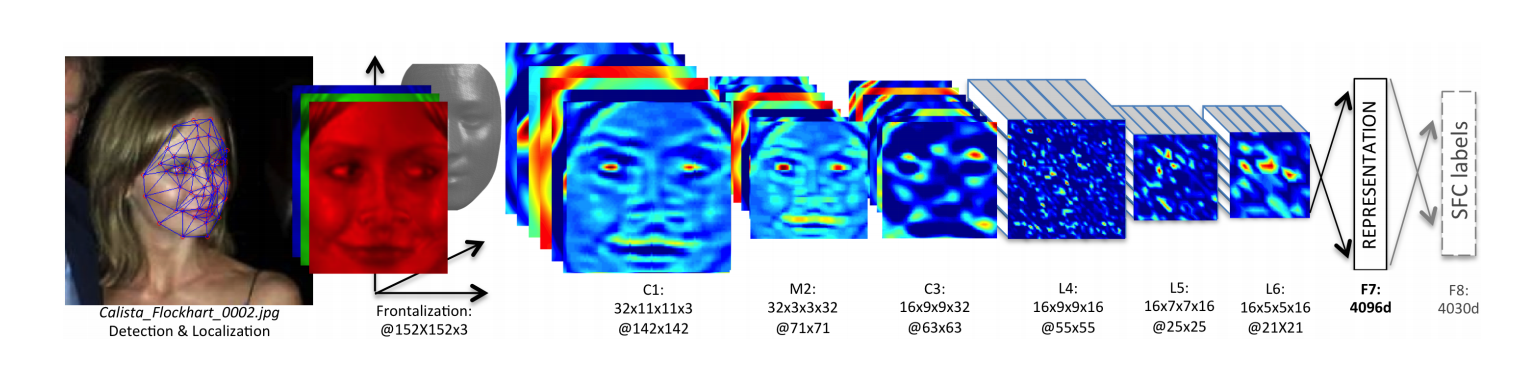
\includegraphics[width=\columnwidth]{images/face-recognition/deepface.png}
    \caption{Outline of DeepFace architecture~\cite{DeepFace}}
    \label{fig:deepface}
\end{figure}

There are 9 layers in the model with over 120 million parameters.
The process of classification is visualized in the picture~\ref{fig:deepface}.
The model was trained on more than 4 million images and as the name of the research paper~\cite{DeepFace} implies, the
results (\textbf{97.35\%} on LFW dataset) almost matched the results of humans (\textbf{97.53\%} on LFW dataset).


\subsubsection{FaceNet}\label{subsubsec:facenet}
FaceNet~\cite{FaceNet} is a system developed by researchers from Google Inc. in 2015.

Interesting innovation of FaceNet lies in the format of its output.
The output of the network is a vector representing a position in an euclidean space (so called embeddings) instead of a
number representing identity.
This approach allows for straight-forward implementation of \textit{verification} and
\textit{identification}~\ref{ch:face-rec}.
Implementation of verification involves thresholding the distance between two embeddings; and identification becomes
k-NN classification problem.

\begin{figure}[H]
    \centering
    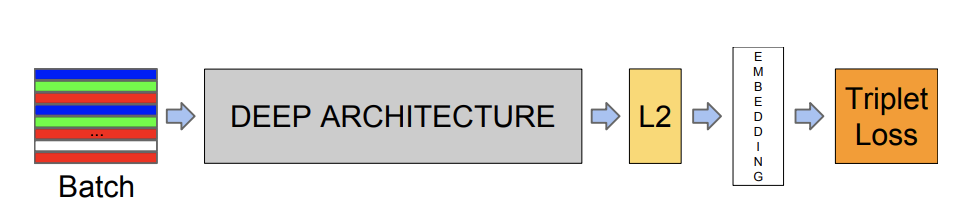
\includegraphics[width=\columnwidth]{images/face-recognition/facenet.png}
    \caption{Outline of FaceNet architecture~\cite{FaceNet}}
    \label{fig:facenet}
\end{figure}

The loss function used to train the model is called \textit{triplet loss}~\ref{subsubsec:triplet-loss}.
Researches at Google came up with new online method\footnote{Training samples are selected during training.} of which
ensures rising difficulty of triplets as the network trains.

The advantages of the model are its accuracy and the compactness of the face representation.
The accuracy of the model exceeded that of human with \textbf{99.63\%} on LFW dataset and the euclidean space has only
128 dimensions.
Another advantage is that the model achieved great results on faces which are not in ideal position without using any
of the complex 3D modeling techniques (as was the case in DeepFace system~\ref{subsubsec:deepface}).
To use proper terms the system is \textit{pose invariant}.

\subsubsection{ResNet}\label{subsubsec:resnet}
A residual neural network (ResNet)~\cite{ResNet} is an ANN which allows for training of networks which contain tens
of layers.
Training of ANN this deep had been practically impossible before the invention of ResNet due to the problem of
\textit{vanishing gradient}\footnote{See footnote on page~\pageref{foot:vangrad}} and \textit{degradation problem}.
The first problem is exposed as a lack of convergence and the second one as a high training error.

Both of these problems have been avoided by implementation of \textit{skip connections} which are illustrated in
figure~\ref{fig:ResNet}.

\begin{figure}[H]
    \centering
    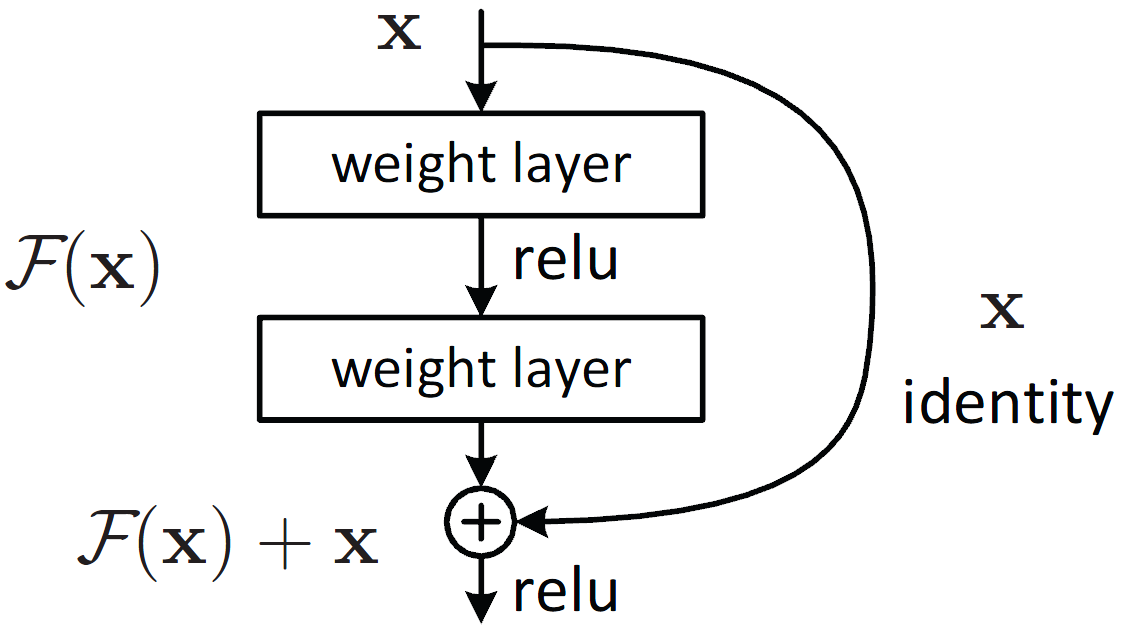
\includegraphics[width=0.9\columnwidth]{images/face-recognition/resnet.png}
    \caption{Residual learning~\cite{ResNet}}
    \label{fig:ResNet}
\end{figure}

The skip connections let the in-between layers fit a residual mapping.
This has proven to be an effective way of using deep neural networks to increase accuracy.

ResNets are widely used in the field of facial recognition as well as in the field of computer vision as a whole.

\subsubsection{InceptionNet}\label{subsubsec:inceptionnet}
InceptionNets are a class of models in which there are multiple kernel sizes operating at the same level.
This is desirable because the right kernel size is dependent on how globally the information is distributed.
A large kernel is preferred when the information is distributed globally and vice versa.

\begin{figure}[H]
    \centering
    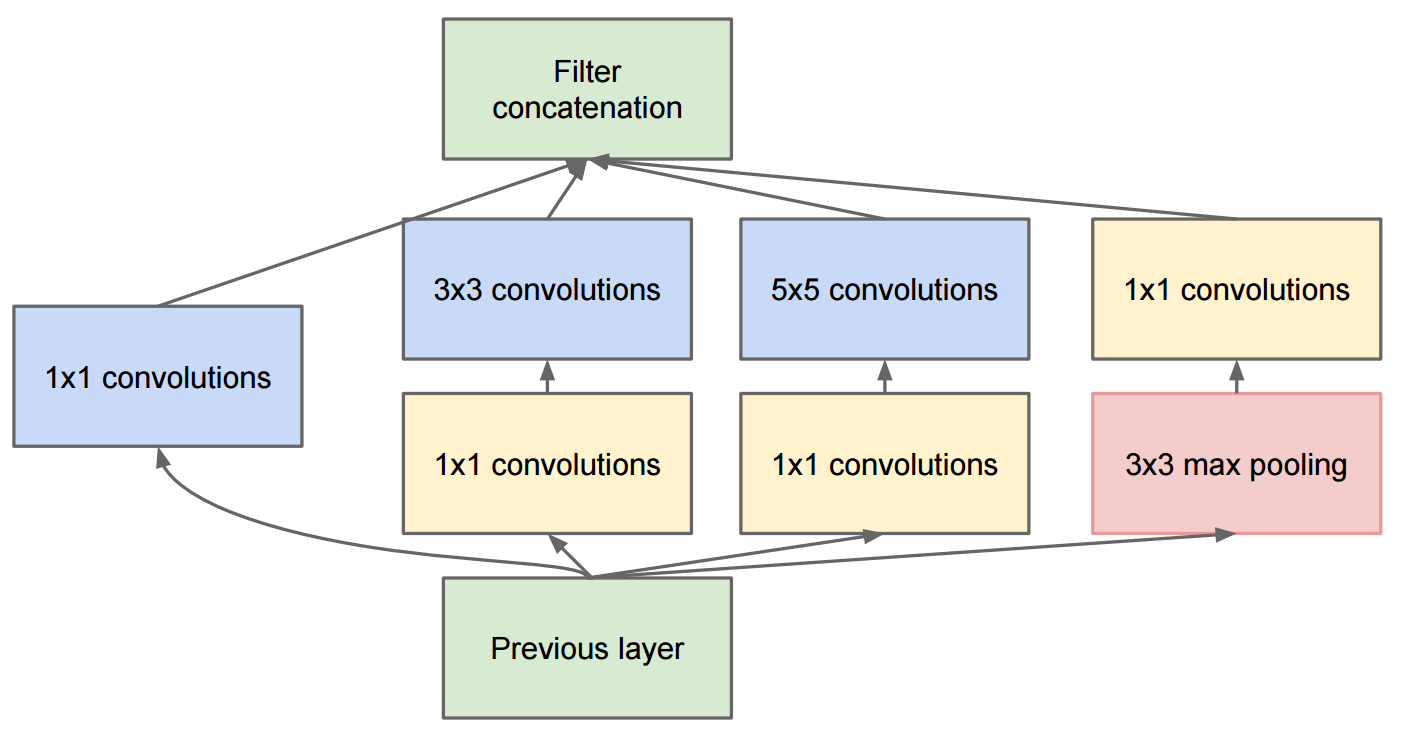
\includegraphics[width=0.9\columnwidth]{images/face-recognition/inceptionnet.png}
    \caption{InceptionNet block~\cite{GoingDeeper}}
    \label{fig:InceptionNet}
\end{figure}

The inception of the inception block (figure~~\ref{fig:InceptionNet}) took place in 2014 in the paper~\cite{GoingDeeper}
published by Google Inc.
Models using inception blocks kept on improving and at the time of writing there is fourth version in use.

\subsubsection{DenseNet}\label{subsubsec:densenet}
DenseNet~\cite{DenseNet} is a type of CNN~\ref{ch:cnn} which was introduced in 2017.
The difference from regular CNNs is that every layer is connected to all the subsequent layers.
Traditional CNN with \textit{L} layers has exactly \textit{L} connections.
On the other hand DenseNet with the same amount of layers contains $\frac{L\left( L+1 \right)}{2}$ connections.
The block of layers is illustrated in figure~\ref{fig:DenseNet}.

\begin{figure}[H]
    \centering
    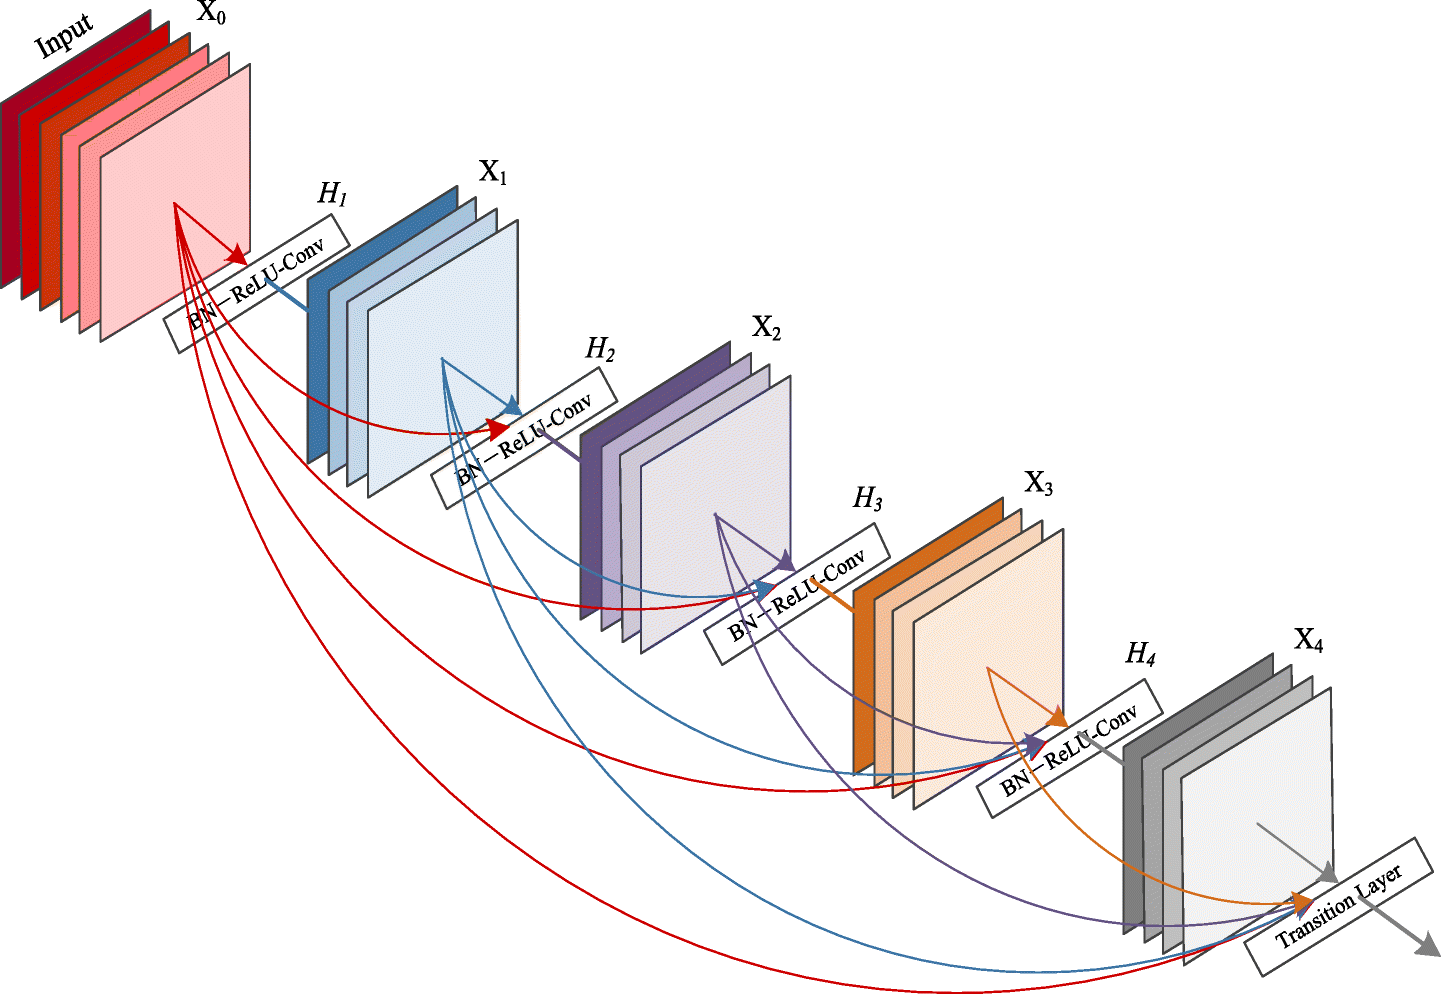
\includegraphics[width=0.9\columnwidth]{images/face-recognition/densenet.png}
    \caption{A 5-layer dense block~\cite{DenseNet}}
    \label{fig:DenseNet}
\end{figure}

DenseNets have several compelling advantages~\cite{DenseNet}.
They alleviate the vanishing-gradient problem, strengthen feature propagation, encourage feature reuse, and
substantially reduce the number of parameters.
\subsection{Loss Functions}\label{subsec:loss-functions}
The main objective of research of loss function is to design a function which leads to a model with superior
discriminative abilities.
How well the model discriminates can be measured by the compactness of clusters and the distance between them.
The goal is for the clusters to be as compact as possible while maximizing the distance in-between them.

\subsubsection{Softmax Loss}\label{subsubsec:softmax-loss}
Softmax~\cite{ArcFace} is the most widely used loss function in general classification tasks and its definition is as
follows:
\begin{equation}
    \label{eq:softmax}
    \mathcal{L}_S = -\frac{1}{N} \sum_{i=1}^{N} \log \frac{e^{W^T_{y_i} x_{i} + b_{y_i}}}
    {\sum_{j-1}^{n} e^{W^T_{j} x_{i} + b_{j}}},
\end{equation}
where $x_i \in \mathbb{R}^{d}$ denotes the feature vector of the \textit{i}-th sample belonging to the $y_i$-th class.
$W_j \in \mathbb{R}^{d}$ is the \textit{j}-th column of the weight matrix $W \in \mathbb{R}^{d \times n}$ and \textit{b}
is the corresponding bias term.
\textit{N} is the batch size and \textit{n} is the class number.

Major drawback of softmax loss is that it doesn't encourage cluster compactness.
In other words, it fails to guarantee similarity among samples within a category.
This makes the learned features not discriminative enough for the open-set face recognition
problem~\footnote{Identifying samples which were not present in the training dataset.}.

The second issue is that the dimension of the output weight matrix grows linearly with the number of identities in the
training set.
This is impractical for large scale deployment.

\subsubsection{Triplet Loss}\label{subsubsec:triplet-loss}
Triplet loss~\cite{TripletLoss} is a loss function which can be optimized by minimizing the distance between
\textit{anchor} and \textit{positive} point while maximizing the distance between \textit{anchor} and \textit{negative}
point.
These points are represented by feature vectors.
The learning process is illustrated in the figure~\ref{fig:tripletloss}.

\begin{figure}[H]
    \centering
    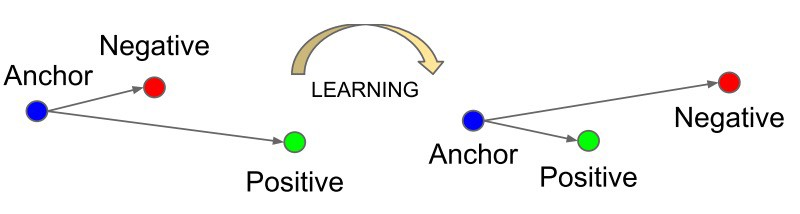
\includegraphics[width=\columnwidth]{images/face-recognition/tripletloss.jpeg}
    \caption{Illustration of the triplet loss~\cite{TripletLoss}}
    \label{fig:tripletloss}
\end{figure}

Anchor and positive points are vectors which belong to the same class whereas negative point belongs to another one.
In the context of facial recognition one class is one identity therefore anchor and positive point are vectorised
representation of two images of one face.

In mathematical terms the loss can be described using Euclidean distance function as follows
\begin{equation}
    \sum_{i}^{N} \left[ \norm{f(x_{i}^{a}) - f(x_{i}^{p}))}^2_2
    - \norm{f(x_{i}^{a}) - f(x_{i}^{n}))}^2_2 + \alpha \right],
\end{equation}
where $f(x_{i}^{a})$, $f(x_{i}^{p})$ and $f(x_{i}^{n})$ are feature vectors of anchor, positive and
negative point of triplet denoted by \textit{i}.
\textit{N} is the number of triplets in the dataset.

The drawbacks of \textit{triplet loss} are the demands entailed by the construction of the triplets.
The number of those is subject to combinatorial explosion and inevitably results in slow convergence and instability
This is a serious issue especially for large datasets.

\subsubsection{Center Loss}\label{subsubsec:center-loss}
The main objective of the research~\cite{CenterLoss} was to design a loss function which solves the main drawbacks of
\textit{sofmax loss}~\ref{subsubsec:softmax-loss} and \textit{triplet loss}~\ref{subsubsec:triplet-loss}.

The discriminative power of the learned features is enhanced by incorporation of the distance of features to the
corresponding class centers.
In other words, the network is penalized whenever the features are too far from the class center.
In the course of training the the centers are updated and the distances of features from centers are minimized.
The model is trained under a joint supervision of softmax loss and center loss.
The effect of these two losses is balanced by a hyperparameter\footnote{A parameter which is not a subject to the
learning process}.
This joint supervision results in a loss function which combines the best of both worlds:
inter-class discriminative power of \textit{softmax loss} and intra-class distance minimization of \textit{center loss}.

The center loss function is intuitively defined by the following equation:
\begin{equation}
    \label{eq:center}
    \mathcal{L}_C = \frac{1}{2} \sum_{i=1}^{m} \norm{x_i - c_{y_i}}_2^2,
\end{equation}
where $c_{y_i} \in \mathbb{R}^{d}$ denotes the $y_i$-th class center of the features.
Recomputing the centers by taking the average of the features over the whole training set id too inefficient and
impractical.

To address this problem the authors proposed updating the centers based on a mini-batch instead of the whole training
set.
To avoid large perturbations caused by mislabeled samples, there is a parameter $\alpha$ with which we control the
learning rate of the centers.

In the equation~\ref{eq:centup} we can see how the center update is computed:
\begin{align}
    \frac{\partial \mathcal{L}_C}{\partial x_i} &= x_i - c_{y_i} \\
    \Delta c_j &= \frac{\sum_{i=1}^m \delta(y_i=j) \cdot (c_j-x_i)}{1+\sum_{i=1}^m \delta(y_i=j)}, \label{eq:centup}
\end{align}
where $\delta(condition)$ is $1$ if the condition is satisfied and $0$ otherwise.

The final loss is described by the following formula:
\begin{equation}
    \label{eq:centerloss}
    \mathcal{L} = \mathcal{L}_S + \mathcal{L}_C = -\sum_{i=1}^{m} \log \frac{e^{W^T_{y_i} x_{i} + b_{y_i}}}
    {\sum_{j-1}^{n} e^{W^T_{j} x_{i} + b_{j}}} + \frac{\lambda}{2} \sum_{i=1}^{m} \norm{x_i - c_{y_i}}_2^2,
\end{equation}

Figure~\ref{fig:centerlosslambda} is a great visualization of the effect of hyperparameter $\alpha$ upon the cluster
compactness.
As is to be expected, higher values of the parameter result in more compact clusters.

\begin{figure}[H]
    \centering
    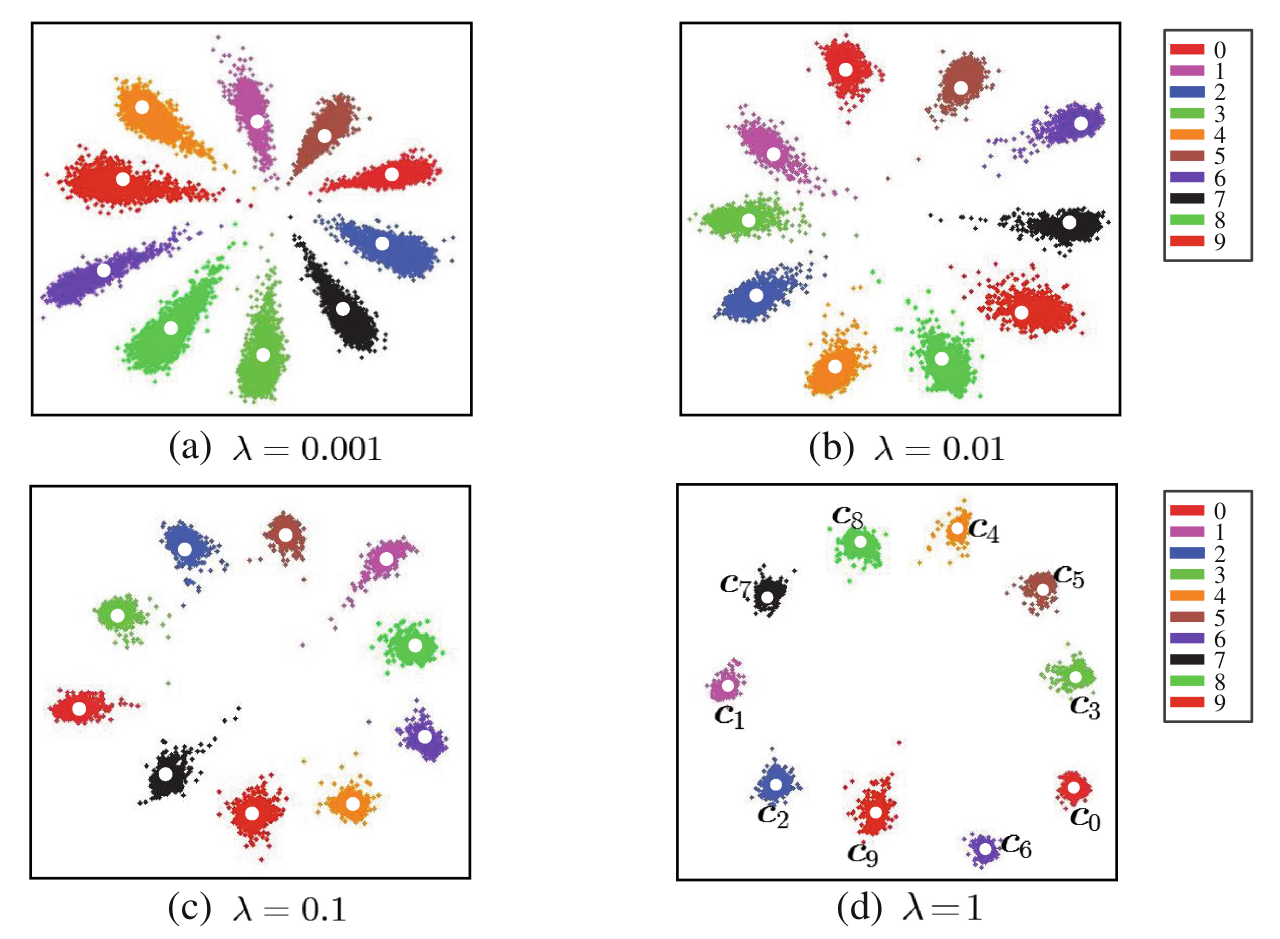
\includegraphics[width=\columnwidth]{images/face-recognition/centerlosslambda.png}
    \caption{Distribution of the features for different values of hyperparameter $\lambda$~\cite{CenterLoss}.
    The white dots $(c_0,c_1,\dots,c_9)$ denote 10 class centers.}
    \label{fig:centerlosslambda}
\end{figure}

\subsubsection{Congenerous Cosine Loss}\label{subsubsec:coco-loss}
Congenerous Cosine Loss~\cite{CocoLoss} (known as COCO loss) is a loss function which was published in 2017.

To define the loss we first have to clarify how the centroid of class \textit{k} is computed.
The centroid\footnote{Center of cluster.} equation is as follows
\begin{equation}
    \boldsymbol{c}_{k} = \frac{\sum_{i \in \beta} \delta \left( l_i, k \right)\boldsymbol{f}^{(i)}}
    {\sum_{i \in \beta} \delta \left( l_i, k \right) + \epsilon} \in \mathbb{R}^{D \times 1},
\end{equation}
where $\beta$ is a mini-batch, $D$ is the feature space dimension, $\delta$ is indicator function, $\epsilon$ is a
trivial number for computation stability, $\boldsymbol{f}^{(i)}$ is the \textit{i}-th feature vector and $l_i$ is
its label.

Now that we have the centroid equation we can define the term we are trying to maximize during model fitting:
\begin{equation}
    p_{l_i}^{(i)} = \frac{exp C(\boldsymbol{f}^{(i)}, \boldsymbol{c}_{l_{i}})}
    {\sum_{k \neq l} exp C(\boldsymbol{f}^{(i)}, \boldsymbol{c}_{k})} \in \mathbb{R},
\end{equation}
where $C$ is standard cosine similarity.

Now we can move on to the final COCO loss function definition:
\begin{equation}
    - \sum_{i \in \beta} \log \left( p_{l_i}^{(i)} \right).
\end{equation}

\subsubsection{SphereFace Loss}\label{subsubsec:sphereface-loss}
SphereFace~\cite{SphereFace} is a loss function which was published in 2018.
The research significantly distinguishes itself from the previously mentioned losses by not relying on euclidean margin.
SphereFace uses angular margin instead.
This has proven to be highly effective in face recognition tasks.

SphereFace loss originates from the softmax loss~\ref{subsubsec:softmax-loss} and its name was inspired by the fact
that the features are projected onto a hypersphere manifold.

To derive SphereFace loss from softmax loss we first incorporate the angle into the softmax equation using the dot
product definition ($a \cdot b = \norm{a} \norm{b} \cos \theta$):

\begin{align*}
    \mathcal{L}_S &= -\frac{1}{N} \sum_{i=1}^{N} \log \frac{e^{W^T_{y_i} x_{i} + b_{y_i}}}
    {\sum_{j-1}^{n} e^{W^T_{j} x_{i} + b_{j}}} \\
    &= -\frac{1}{N} \sum_{i=1}^{N} \log \frac{e^{\norm{W_{y_i}} \norm{x_i} \cos(\theta_{y_i,i}) + b_{y_i}}}
    {\sum_{j-1}^{n} e^{\norm{W_j} \norm{x_{i}} \cos(\theta_{j,i}) + b_{j}}},
\end{align*}
where $\theta_{j,i}$ is the angle between vector $W_j$ and $x_i$.
The meanings of the remaining symbols are equal to those in the softmax equation~\ref{eq:softmax}.


Next we normalize $\norm{W_j} = 1, \forall j$ and set the bias term to 0.
\begin{equation}
    \label{eq:softmaxmod}
    \mathcal{L}_{modified} = -\frac{1}{N} \sum_{i=1}^{N} \log \frac{e^{\norm{x_i} \cos(\theta_{y_i,i})}}
    {\sum_{j-1}^{n} e^{\norm{x_{i}} \cos(\theta_{j,i})}}
\end{equation}
While it's possible to learn features with the modified loss the features are not discriminative enough.
To improve the discriminative power angular margin was incorporated:
\begin{equation}
    \label{eq:ang}
    \mathcal{L}_{ang} = -\frac{1}{N} \sum_{i=1}^{N} \log \frac{e^{\norm{x_i} \cos(m\theta_{y_i,i})}}
    {e^{\norm{x_i} \cos(m\theta_{y_i,i})} + \sum_{j \neq y_i} e^{\norm{x_{i}} \cos(\theta_{j,i})}},
\end{equation}
where $\theta_{y_i,i}$ lies in $\left[ 0, \frac{\pi}{m} \right]$.

The decision boundary for a binary case is defined by:
\begin{equation}
    \label{eq:spherebound}
    \cos{m\theta_1} = \cos{\theta_2},
\end{equation}
where $\theta_i$ is the angle between the feature and weight of class $i$.

To make the loss~\ref{eq:ang} optimizable for CNNs the definition range of $\cos(\theta_{y_i},i)$ is expanded.
This is achieved by replacing the cosine term with monotonically decreasing angle function $\Psi(\theta_{y_i},i)$
\begin{equation}
    \mathcal{L}_{ang} = -\frac{1}{N} \sum_{i=1}^{N} \log \frac{e^{\norm{x_i} \Psi(m\theta_{y_i,i})}}
    {e^{\norm{x_i} \Psi(m\theta_{y_i,i})} + \sum_{j \neq y_i} e^{\norm{x_{i}} \Psi(\theta_{j,i})}}
\end{equation}
The angle function has the following definition:
\begin{equation}
    \Psi(\theta_{y_i,i}) = (-1)^{k} \cos(\theta_{y_{i},i}) -2k,
\end{equation}
where $k \in \left[ 0, m-1 \right]$.
Parameter $m \geq 1$ gives us the control over the angular margin size.

\subsubsection{CosFace Loss}\label{subsubsec:cosface}
CosFace~\cite{CosFace} is another loss using margin to achieve better discriminative power than
softmax~\ref{subsubsec:softmax-loss}.

The decision boundary for binary case is defined by the following equation:
\begin{equation}
    \label{eq:cosbounary}
    \cos{\theta_1} - m = \cos{\theta_2},
\end{equation}
where the symbols have exactly the same meaning as in the equation~\ref{eq:spherebound} of SphereFace decision boundary.
The advantage of CosFace over SphereFace is the ease of optimization.
The reason for that is that the decision boundary of CosFace is not being defined over the angular space.
Optimization in angular space is more difficult because of the non-monotonicity of the cosine function.

Another innovation over SphereFace is that not only is the weight vector $W_j$ normalized, but the feature vectors
$x_i$ as well.
This achieves much lower intra-class variability by concentrating more on the angle during training.
By fixing $\norm{x}$ as some predetermined radius $s$ in equation~\ref{eq:softmaxmod} we get:
\begin{equation}
    \mathcal{L}_{ns} = -\frac{1}{N} \sum_{i=1}^{N} \log \frac{e^{s \cos(\theta_{y_i,i})}}
    {\sum_{j-1}^{n} e^{s \cos(\theta_{j,i})}}
\end{equation}
This loss is called Normalized Softmax Loss (NSL) in the CosFace research paper.
NSL emphasizes correct classification but is not discriminative enough for face recognition tasks.
For this reason (as was mentioned in the SphereFace research as well) the margin is incorporated:
\begin{equation}
    \label{eq:cosface}
    \mathcal{L}_{lmc} = -\frac{1}{N} \sum_{i=1}^{N} \log \frac{e^{s \left( \cos(\theta_{y_i,i}) - m \right)}}
    {e^{s\ \left( \cos(\theta_{y_i,i}) - m \right)} + \sum_{j \neq y_i}^n e^{s\ \cos(\theta_{j,i})}},
\end{equation}
subject to
\begin{align}
    W &= \frac{W*}{\norm{W*}}, \\
    x &= \frac{x*}{\norm{x*}}, \\
    \cos(\theta_j, i) &= W_{j}^T x_i.
\end{align}
The meaning of the equation constituents is equivalent to those in the previous sections.

The equation~\ref{eq:cosface} is the final form of the CosFace loss.
The authors of the research call it the Large Margin Cosine Loss (LMCL).

\subsubsection{ArcFace Loss}\label{subsubsec:arcface}
ArcFace loss is used in this thesis which makes it the topic of the following chapter~\ref{ch:arcface}.

    \chapter{ArcFace}\label{ch:arcface}
ArcFace~\cite{ArcFace} is a research which became public in 2018 and achieved state-of-the-art results on LFW dataset.

ArcLoss is based on the equation of \textit{softmax loss}~\ref{eq:softmax}.
There are few steps separating the original and the improved version:
\begin{enumerate}
    \item First step is to fix the bias $b_j = 0$.
    \item Then we transform the logit using the dot product definition $W_j^T x_i = \norm{W_j} \norm{x_j} \cos \theta_j$
    $\theta$ is the angle between the weight $W_j$ and the feature $x_i$.
    \item In a third step we fix the individual weights $\norm{W_j} = 1$ by $l_2$ normalization
    \item We do the same for feature $x_i$ and re-scale it to $s$ where coefficient $s$ is predetermined feature scale.
    These normalization steps make the prediction depend only on the angle $\theta$.
    The embeddings are distributed on the hypersphere with a radius $s$.
\end{enumerate}

\begin{figure}[H]
    \centering
    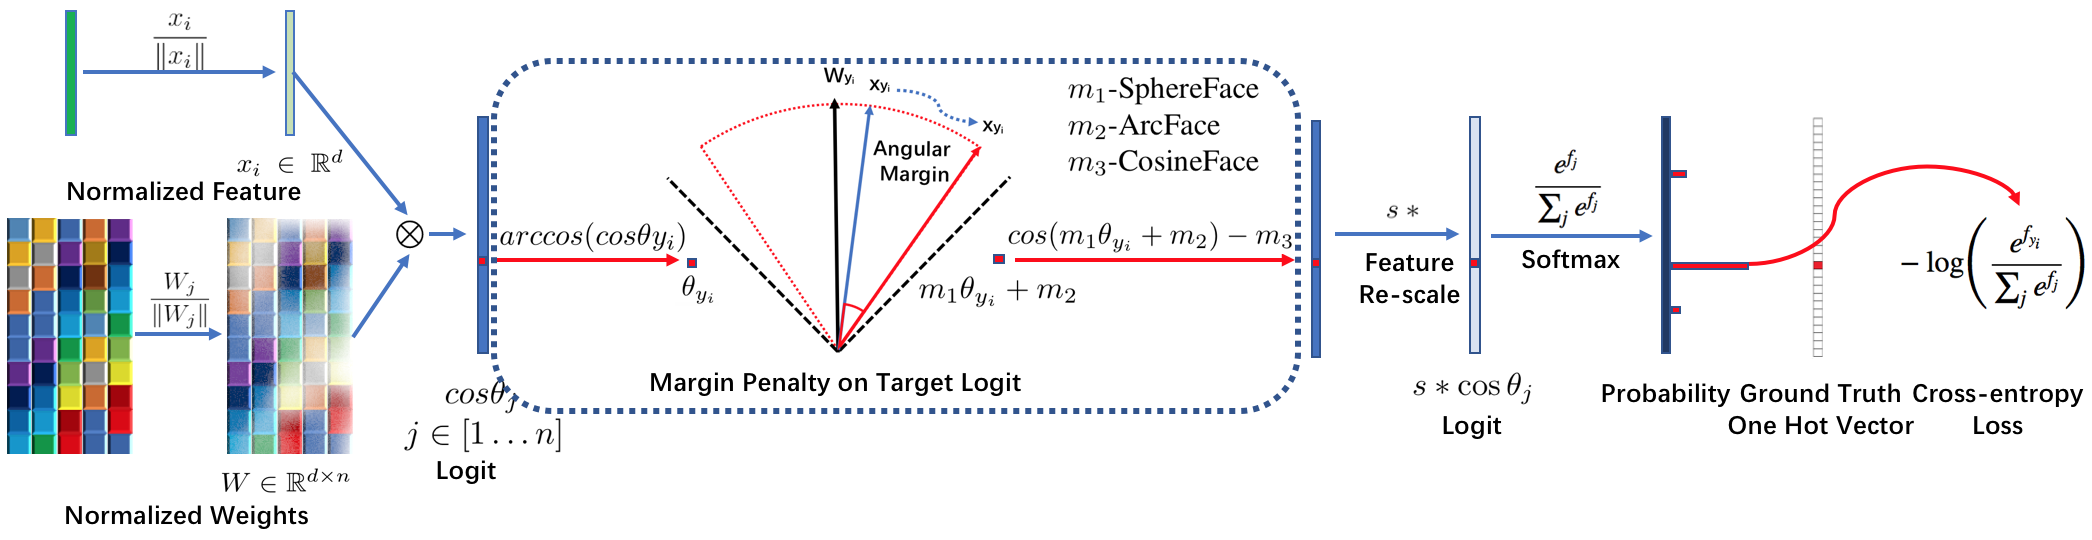
\includegraphics[width=\columnwidth]{images/arcface/arcface.png}
    \caption{Training a CNN for face recognition supervised by the ArcFace loss~\cite{ArcFace}}
    \label{fig:arcface}
\end{figure}

At this point the loss function equation is as follows:
\begin{equation}
    \mathcal{L} = -\frac{1}{N} \sum_{i=1}^{N} \log \frac{e^{s \cos(\theta_{y_i,i})}}
    {e^{s\ \cos(\theta_{y_i,i})} + \sum_{j = 1, j \neq y_i}^n e^{s\ \cos(\theta_{j,i})}}.
\end{equation}

\begin{enumerate}
    \setcounter{enumi}{4}
    \item Now we incorporate the additive margin penalty \textit{m} between $x_i$ and $W_{y_i}$.
    The angluar margin is equal to the geodesic distance\footnote{Distance of a curve representing shortest path
    between two points in a surface.} on the hypersphere which is the reason why the method is called
    \textit{ArcFace}.
\end{enumerate}

Final ArcFace loss function:
\begin{equation}
    \mathcal{L} = -\frac{1}{N} \sum_{i=1}^{N} \log \frac{e^{s \cos(\theta_{y_i,i} + m)}}
    {e^{s\ \cos(\theta_{y_i,i} + m)} + \sum_{j = 1, j \neq y_i}^n e^{s\ \cos(\theta_{j,i})}}.
\end{equation}

\section{Comparison with SphereFace and CosFace}\label{sec:arc-comparison}
By having a look at figure~\ref{fig:arcfacecomp} we can do a comparison of geometric differences of decision margins.
The advantage of \textit{ArcFace} is its constant linear angular margin throughout the whole interval.

\begin{figure}[H]
    \centering
    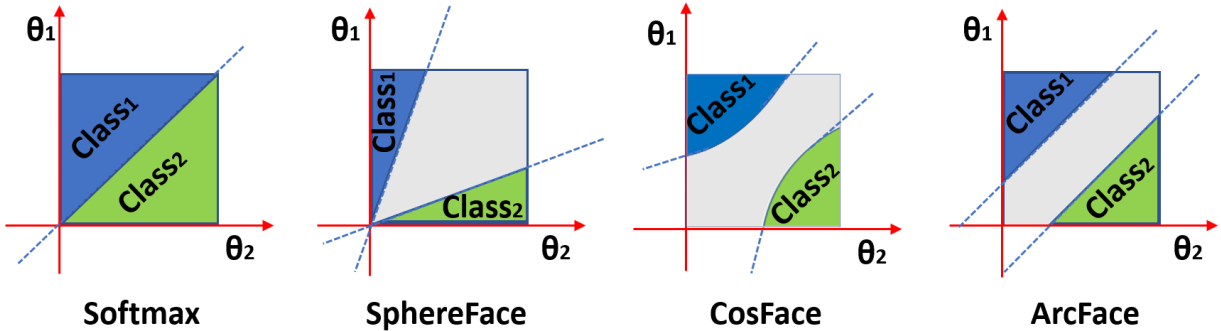
\includegraphics[width=\columnwidth]{images/arcface/arcfacecomparison.png}
    \caption{Decision margins of different loss functions under binary classification case.~\cite{ArcFace}}
    \label{fig:arcfacecomp}
\end{figure}

We can see the concrete results in table~\ref{tbl:arcfacecomp}.
ResNet100 with ArcFace loss trained on MS1MV2~\ref{subsec:ms1m} dataset exceeded the results of methods mentioned in
this thesis.

\begin{table}[H]
    \begin{tabularx}{\textwidth}{l|XXc}
        Method                & \#Image & LFW~\ref{subsec:lfw}            & YTF~\ref{subsec:ytf}            \\ \hline
        FaceNet~\ref{subsubsec:facenet}               & 200M    & 99.63          & 95.10          \\
        Center Loss~\ref{subsubsec:center-loss}           & 0.7M    & 99.28          & 94.90          \\
        SphereFace~\ref{subsubsec:sphereface-loss}            & 0.5M    & 99.42          & 95.00          \\
        CosFace~\ref{subsubsec:cosface}               & 5M      & 99.73          & 97.60          \\
        MS1MV2, R100, ArcFace & 5.8M    & \textbf{99.83} & \textbf{98.02}
    \end{tabularx}
    \caption{Verification performance (\%) of different methods on LFW and YTF datasets.}
    \label{tbl:arcfacecomp}
\end{table}

    \chapter{Evaluation Metrics}\label{ch:evaluation-metrics}
In this chapter, I will define metrics used for performance evaluation.

Before doing so, it is necessary to describe constituents of the confusion matrix~\ref{fig:confusionmat}.

\begin{figure}[H]
    \centering
    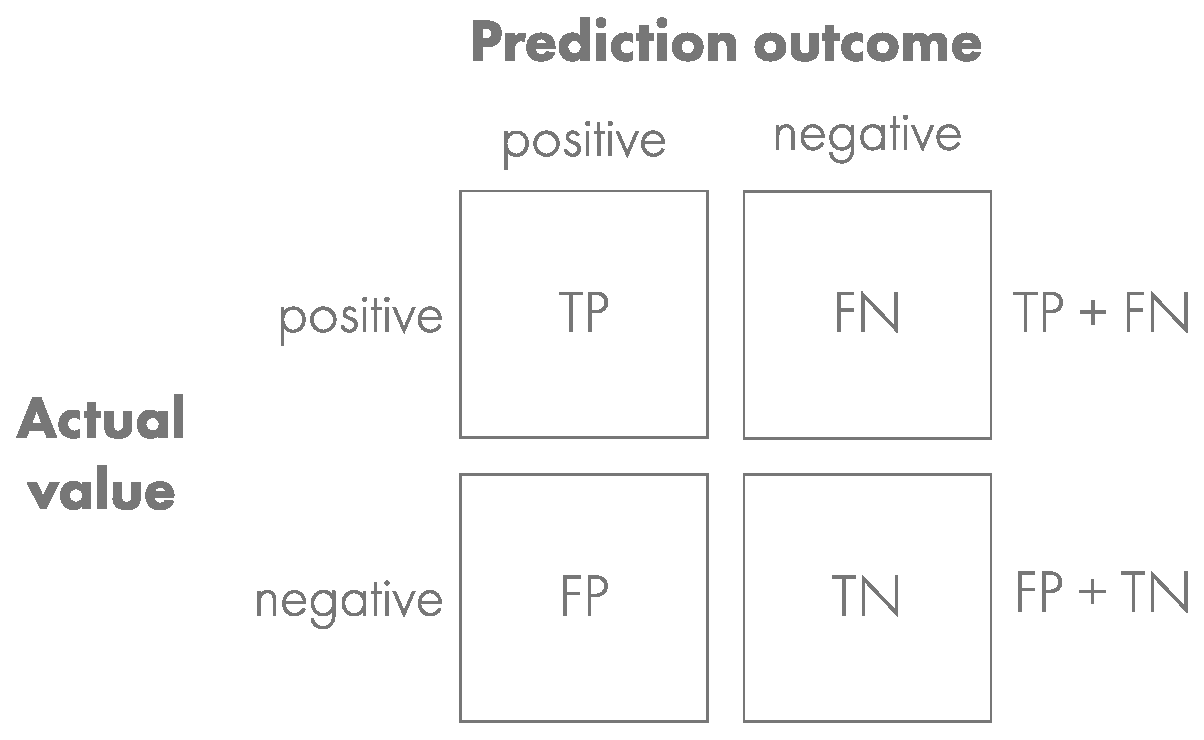
\includegraphics[width=0.9\columnwidth]{images/implementation/confusion_matrix.eps}
    \caption{Confusion matrix~\cite{ConfMat}}
    \label{fig:confusionmat}
\end{figure}

\textbf{True Positives} (TP) is the number of actual positives being predicted as positive.

\textbf{False Positives} (FP), also known as \textbf{type I error}, is the number of actual negatives being predicted
as positive.

\textbf{False Negatives} (FN) is the number of actual positives being predicted as negative.
FN is called \textbf{type II error}.

\textbf{True Negatives} (TP) is the number of actual negatives being predicted as negative.

With these terms introduced, we can proceed with a definition of precision~\ref{sec:precision} and
recall~\ref{sec:recall}.

\section{Precision}\label{sec:precision}
Precision~\cite{PreRec} is the number of relevant instances among the retrieved instances.
Mathematically speaking, precision is defined as the following fraction:
\begin{equation}
    Precision = \frac{TP}{TP + FP},
\end{equation}
where TP and FP are the constituents of the confusion matrix~\ref{fig:confusionmat}.

A useful feature of precision is that it can be used to detect faulty model and dataset mislabelings.
This property was extensively used during system implementation~\ref{ch:implementation}.

\section{Recall}\label{sec:recall}
Recall~\cite{PreRec} (also called sensitivity) is the fraction of the total amount of relevant instances that were
actually retrieved.
A definition of recall is the following:
\begin{equation}
    Recall = \frac{TP}{TP + FN},
\end{equation}
TP and FN were described in the beginning of the chapter.

\section{$F_1$-score}\label{sec:f-score}
$F_1$-score is the harmonic mean of precision and recall.
The metric is defined by the following formula:
\begin{equation}
    F_1 = 2 \cdot \frac{precision \cdot recall}{precision + recall}.
\end{equation}

The important property of this metric is that it successfully deals with skewed data.
This scenario occurs when there is much more positives than negatives in the data or vice versa.
A typical example is a classifier used to diagnose a rare illness.
If the model always predicted false, the accuracy\footnote{Sum of true positives divided by the number of predictions.}
would be high even though the system would be essentially useless.

    \chapter{System Design and Implementation}\label{ch:implementation}
The system pipeline\footnote{See footnote on page~\pageref{foot:pipe}} consists of three separate processes:
data preprocessing~\ref{sec:data-preprocessing}, feature extraction~\ref{sec:feature-extraction} and
evaluation~\ref{sec:evaluation}.

The system is implemented in \textit{Python} programming language.
Libraries \textit{NumPy} and \textit{PyTorch} are being extensively used throughout the whole pipeline.

\section{Data Preprocessing}\label{sec:data-preprocessing}
\begin{wrapfigure}[7]{r}{0pt}
    \centering
    \raisebox{0pt}[\dimexpr\height-0.831\baselineskip\relax]{%
    \begin{forest}
        for tree={
        font=\ttfamily,
        grow'=0,
        child anchor=west,
        parent anchor=south,
        anchor=west,
        calign=first,
        edge path={
        \noexpand\path [draw, \forestoption{edge}]
        (!u.south west) +(7.5pt,0) |- node[fill,inner sep=1.25pt] {} (.child anchor)\forestoption{edge label};
        },
        before typesetting nodes={
        if n=1
        {insert before={[,phantom]}}
        {}
        },
        fit=band,
        before computing xy={l=15pt},
        }
        [dataset
        [name1
        [image1\_128x128.jpg]
        [image2\_128x128.jpg]
        [image3\_128x128.jpg]
        ]
        [name2
        [image1\_128x128.jpg]
        [image2\_128x128.jpg]
        ]
        [\ldots]
        ]
    \end{forest}
    }
    \caption{Standard image dataset format}
    \label{fig:dataset}
\end{wrapfigure}
The goal of preprocessing is to convert the input dataset~\ref{subsec:dataset-description} to a standard format.
The standardized dataset consists of directories with each directory representing one identity/label.
In these directories there are images corresponding to the identity.
In this case, the images contain faces in different positions.

The desired format is visualized in figure~\ref{fig:dataset}.

\subsection{Dataset Description}\label{subsec:dataset-description}
The input dataset consists of 15 videos and the same amount of annotation files in \textit{json}\footnote{An
open-standard file format that uses human-readable text to transmit data objects consisting of attribute–value pairs
and array data types.} format.

In every annotation file there is a dictionary object, where key is a name and value is a list of detections.
Every detection contains information about frame and the position of the face.
This information is used to transform the dataset to standardized format.
The reference face position was selected by human.
Because of that, the geometry of the area is not always consistent which significantly decreases the model performance.
For this reason, as is described in the following section~\ref{subsec:preproalgo}, this reference position is not
used directly in the algorithm.

\subsection{Preprocessing Algorithm}\label{subsec:preproalgo}
Before the presentation of the algorithm it is necessary to define "Intersection over Union (IoU)."
As the name implies IoU is computed as a fraction with intersection area in the numerator and union area in the
denominator (see figure~\ref{fig:iou}).

\begin{figure}[H]
    \centering
    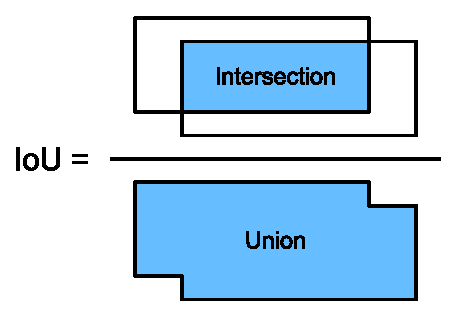
\includegraphics{images/implementation/iou.eps}
    \caption{IoU visualization\cite{IoU}}
    \label{fig:iou}
\end{figure}

The preprocessing algorithm consists of seven steps:
\begin{enumerate}
    \item First I iterate over the annotation files.
    \item Then I iterate over the names and detections within the file.
    \item In the third step I fetch the frame out of the video corresponding to the detection.
    \item Then I detect all the faces in the frame using MTCNN detector.
    The detector returns coordinates of the bounding boxes\footnote{See footnote on page~\pageref{foot:bbox}} and the
    facial landmarks\footnote{Salient regions of the face.}.
    \item I select the detection which meets the following two conditions:
    \begin{enumerate}
        \item has the biggest IoU with the bounding box from the annotation file of all the detections;
        \item the IoU value is at least \textbf{0.5} (This value has been determined experimentally as
        is described in the section~\ref{subsec:detection-mislabelings}.).
    \end{enumerate}
    In case these two conditions are not met for any of the detections the frame is omitted.
    \item Now I perform face frontalization using the facial landmarks from the previous steps and the predetermined
    position of target facial landmarks.
    This is achieved by using the least squares method to find an affine transformation\footnote{A function between
    affine spaces which preserves points, straight lines and planes.} between the two sets of coordinates.
    After the transformation the image geometry is 128x128 and the facial landmarks are in the same position across
    the whole dataset.
    \item In the last step I save the transformed image on the path defined by the standardized dataset format
    (\path{dataset/name/image_128x128.jpg}).
\end{enumerate}

Having the dataset in the desired format we can proceed with feature extraction.

\section{Feature Extraction}\label{sec:feature-extraction}
Feature extraction~\cite{FeEx} is a process of dimensionality reduction by which an initial set of raw data
is reduced to the set of feature vectors.
In this study this process is carried out by feeding the input image $x_i \in \mathbb{R}^{128\times128 }$ to the CNN model.
On the output we retrieve a feature vector $y_i \in \mathbb{R}^{1024}$.

The model used is 18 layer ResNet~\ref{subsec:resnet} which was trained under a supervision of the ArcFace loss.
The training process was not carried out as part of this thesis.
The pretrained model was downloaded from the ArcFace implementation repository~\cite{ArcFacePyTorch}.

\subsection{Feature Extraction Algorithm}\label{subsec:feexalgo}
The feature extraction algorithm consists of 6 steps:
\begin{enumerate}
    \item Initially I will iterate over the images in the dataset.
    \item In the second step I save the image and the flipped version into an array
    with shape $2\times1\times128\times128$.
    \item With this shape, the array can be put on the inputs of ResNet-18.
    \item I retrieve the feature vector on the output.
    \item In the fifth step the vector along with the corresponding label is saved into an array.
    \item Once all the feature vectors are computed, the resulting array is saved using \textit{h5py} module.
\end{enumerate}

In the final array there are 478529 feature vectors.
The whole file is approximately 2 GB in size.

Having the feature vectors computed we can carry out evaluation~\ref{sec:evaluation}.

\section{Evaluation}\label{sec:evaluation}
The system's performance is evaluated on the verification task.
To describe the algorithm in simple words, the task consists of computing cosine distance between every two feature
vectors and deciding, given some threshold, whether the vectors correspond to the same identity ot not.
This computation is carried out for all the threshold values in the specified interval.

The algorithm is described in depth in the following section~\ref{subsec:thresholding-algorithm}.

\subsection{Thresholding Algorithm}\label{subsec:thresholding-algorithm}
First I would like to analyze the algorithm time complexity and memory demands.

As I previously mentioned, it is necessary to compute the distances between every two feature vectors in the dataset.
The number of vector pairs is equal to
\begin{equation}
    N_{pairs} = \frac{n\left(n+1\right)}{2} = \frac{478529\left(478529+1\right)}{2} \approx 114.50 \cdot 10^9,
\end{equation}
where $n = 478529$ is the number of vectors in the dataset.
If we computed all the distances at once using optimized matrix operations we would need at least 460 GB of RAM memory.

Given that the algorithm time complexity is $O(n^2)$ and the big memory demands it was desirable to split the distance
matrix into smaller sub-matrices.
These sub-matrices than could be submitted to different CPU cores to process which significantly reduced the computation
time.
This approach made the use of optimized matrix libraries possible while reducing the excessive memory demands.

There are 5 steps in the parallelized algorithm:
\begin{enumerate}
    \item Initially I generate all the interval pairs.
    \item In the second step I pass the intervals as an argument to the generator function.
    This function returns pairs of slices of the feature vector array and corresponding labels.
    \item Next I pass the generator function as an argument to the \textit{imap} method from \textit{multiprocessing}
    module.
    This method iterates over the generator function and passes the retrieved values to separate processes.
    With this step, parallelized processing is achieved.
    \item In the fourth step the matrix of cosine distances is computed between the two feature vector arrays
    and two label arrays using \textit{cosine\_distances} method from \textit{sklearn} library.
    Computing the matrix for labels allows for simple and efficient comparison of predictions and reference
    values using matrix operations.
    \item Next I convert the matrices to two long vectors.
    \item Now I iterate over the list of threshold values ($\left[ 0, 0.05, 0.10, 0.15, \ldots 2 \right]$).
    \item I apply the threshold to the distances.
    This way I retrieve a vector of binary values.
    \item I use the methods \textit{sum} and \textit{logical\_and} along with elementwise binary value inversion to
    count the number of \textit{true positives (TP)}, \textit{true negatives (TN)}, \textit{false positives (FP)} and
    \textit{false negatives (FN)}.
    \item In the last step I do elementwise summation of the arrays which were returned from the processes.
\end{enumerate}

The output of the algorithm is an array with 200 rows and 4 columns.
The rows correspond to the threshold values; columns to \textit{TP}, \textit{TN}, \textit{FP} and \textit{FN}.

Having all these values accumulated we can proceed with computation of all the relevant metrics.

\subsection{Performance Comparison}\label{subsec:performance-comparison}
In order to evaluate the performance I implemented an algorithm which computes precision~\ref{sec:precision},
recall~\ref{sec:recall} and $F_1$ score~\ref{sec:f-score} on the data from previous section.

In figure~\ref{fig:prft} we can see the progression of these metrics.

\begin{figure}[H]
    \begin{subfigure}{\textwidth}
        \centering
        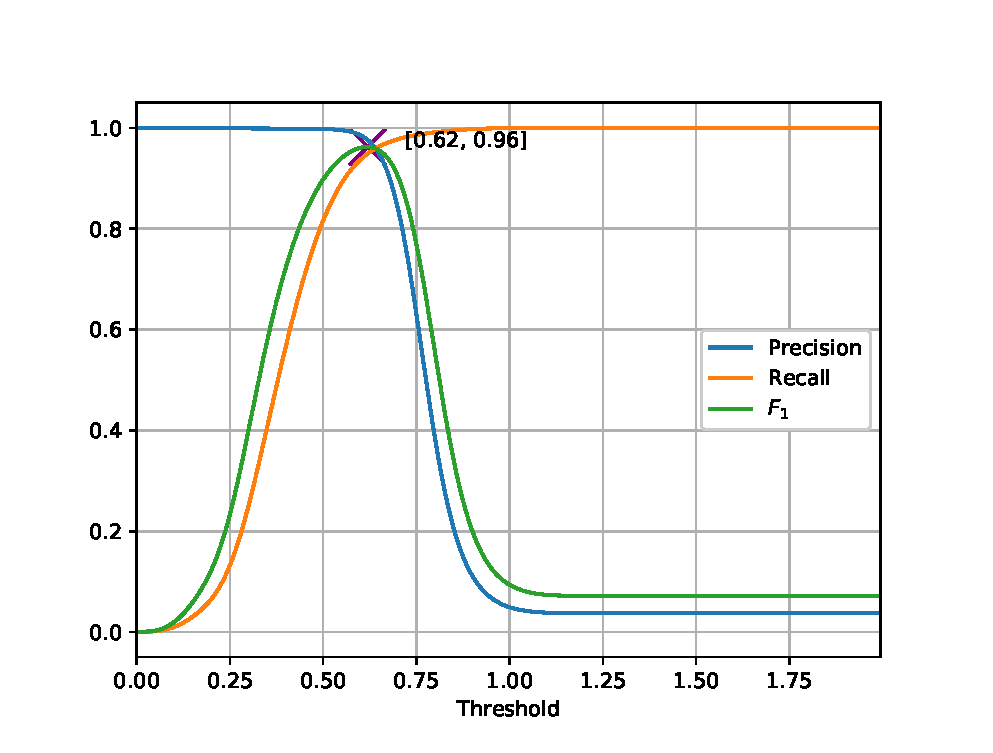
\includegraphics[width=0.95\columnwidth]{images/implementation/prft_fav-128_N1.eps}
        \caption{ResNet-18 trained under a supervision of ArcFace loss function}
        \label{fig:prft_arcface}
    \end{subfigure}%

    \begin{subfigure}{\textwidth}
        \centering
        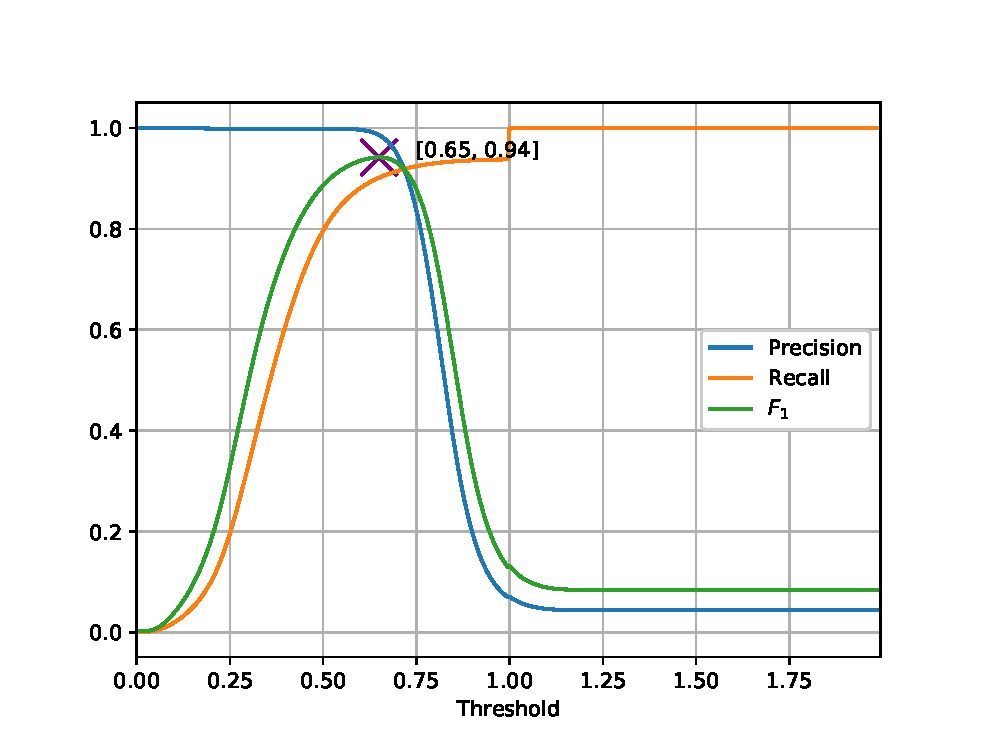
\includegraphics[width=0.95\columnwidth]{images/implementation/prft_eyedea.eps}
        \caption{Commercial system developed by Eyedea Recognition s. r. o.}
        \label{fig:prft_eyedea}
    \end{subfigure}
    \caption{Progression of precision, recall and $F_1$ score with increasing threshold values.}
    \label{fig:prft}
\end{figure}

\subsection{Detection of Mislabelings}\label{subsec:detection-mislabelings}
As I mentioned in the section~\ref{sec:precision}, precision curve can be used to detect incorrect labels in the
dataset.
In figure~\ref{fig:faulty_prft} there are three functions dependent on threshold.

\begin{figure}[H]
    \centering
    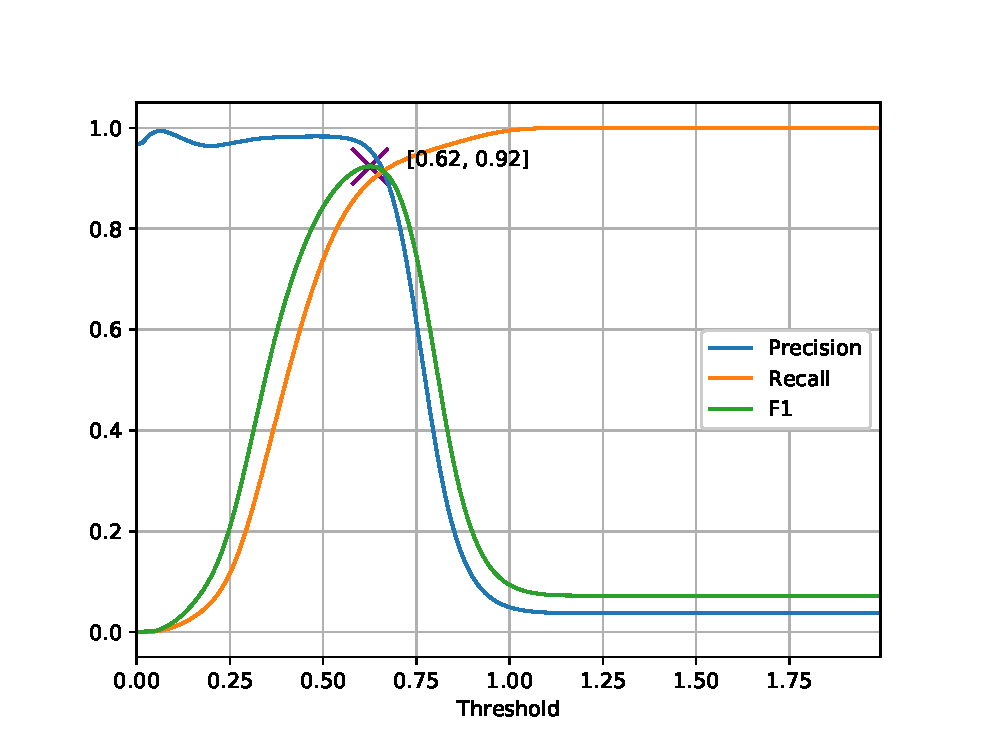
\includegraphics[width=0.95\columnwidth]{images/implementation/faulty_prft.eps}
    \caption{An example of precision curve~\ref{sec:precision} computed on a dataset containing errors.}
    \label{fig:faulty_prft}
\end{figure}

By the definition of precision ($Precision = \frac{TP}{TP+FP}$), there should not be any false positives
for threshold 0 because in such a setting, the system is strongly biased towards false negatives.
With this in mind, value of precision which is not equal to 1 for threshold 0 is a sign that there are either
mislabelings in the dataset or that the whole model is faulty.

\begin{figure}[H]
    \centering
    
\includegraphics[width=0.9\columnwidth]{images/implementation/faulty_detection.jpg}
    \caption{An example of a faulty detection.}
    \label{fig:faulty_bbox}
\end{figure}

This idea was used extensively during the experimentation.
Figure~\ref{fig:faulty_bbox} is an example of faulty face detection.
Because of the white stripe, the man in the foreground was not detected by the MTCNN detector selecting the bald man
on the right instead.
This led to an error in the dataset and it is the reason why the IoU threshold was put in place during the data
preprocessing~\ref{sec:data-preprocessing}.

\subsection{Face Detector Evaluation}\label{subsec:detectorevaluation}
In order to evaluate the detector I've implemented an algorithm which computes recall~\ref{sec:recall} on the IoU
values between the MTCNN detection and the area selected by human.
The process is very similar to the one described in section~\ref{subsec:thresholding-algorithm}.

The output is visualized in the image~\ref{fig:iou}.

The fact that recall ($\frac{TP}{TP+FN}$) never gets close to 1 is indicative of significant amount of
\textit{false negatives}.
To say it in other words, there are plenty of cases in which the face is not detected at all.

The value marked by purple cross is the threshold value set in the data processing pipeline~\ref{subsec:preproalgo}.
The big drop in recall for thresholds in range $\left< 0.4, 0.5 \right>$ is caused by not accepting the detections
of neighboring faces~\ref{fig:faulty_bbox} as \textit{true positive}.
With this in mind, higher recall value doesn't necessarily mean better performance.

\begin{figure}[H]
    \centering
    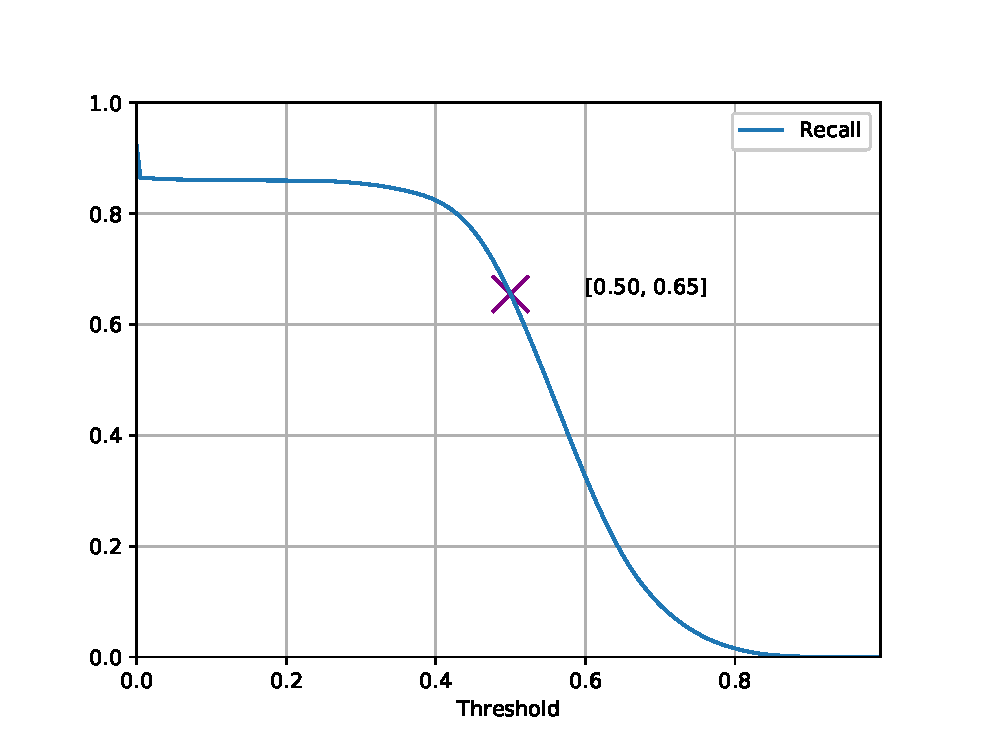
\includegraphics[width=0.95\columnwidth]{images/implementation/mtcnn_recall_fav-128_N1.eps}
    \caption{Recall computed on IoU~\ref{fig:iou} values.}
    \label{fig:mtcnn_recall}
\end{figure}

The selection of neighboring face as \textit{true positive} is exacerbated by the penchant of humans to select larger
area as containing the face.
To verify this hypothesis I implemented a script which computes the average ratio of the area selected by human
to that of the detector.
The resulting ratio is \textbf{1.59}.
This means that human selects on average an area which is \textbf{59 \% larger} than the one selected by the detector.

    \chapter{Conclusion}\label{ch:conclusion}
In the introduction~\ref{sec:goals} I stated goals of this study.

The main objective was to implement state-of-the-art algorithm and compare its performance with a commercial system.
Given that the performance of my system exceeded that of commercial one by two percents I dare to say that the
goal of this thesis was accomplished.

\section{Possible Improvements}\label{sec:possible-improvements}
I have two ideas which could lead to the improvements in system's performance:
\begin{itemize}
    \item \textit{Fitting the model on relevant identities.} The model used at the core of the system (ResNet-18) was
    fitted on identities which are not relevant in the context of the system's application.
    While this is not an issue as the model works well on open-set\footnote{See footnote on page~\pageref{foot:openset}}
    problems, training the model again is one way to improve the system.
    \item \textit{Better face detection engine.} An area where the system is lacking is the face detection engine.
    The detector available in the Eyedea SDK seems to be significantly more robust than the one used in this work.
    This manifested itself when looking at the images of faulty MTCNN detection (see~\ref{fig:faulty_bbox}).
    Eyedea detector is better at handling edge cases (e.g. white stripe over part of the face).
    Such edge cases lead to MTCNN producing false negatives.
\end{itemize}

%    \setquotestyle{english} % Question marks in place of quotes bug fix
    \printbibliography

\end{document}